\chapter{Psychological Well-being and Demographic Factors can Mediate Soundscape Pleasantness and Eventfulness}
\label{ch:whostudy}
\draft{The orange highlighted sections are those which I am potentially concerned about being too similar to Mercede's work or weren't sections I wrote in the original paper. I would highly prefer to be able to leave them in as is, and I'm hoping the context and footnotes provided are enough to make this possible.}

\section{Introduction}

\copied{Understanding of soundscape perception is intimately tied to certain key factors known as primary factors of soundscape perception comprising acoustic properties (physical features) of the sound such as frequency/pitch \citep{Kumar2008Mapping} and intensity/loudness \citep{Kaya2020Pitch} and secondary influences like emotions and personality traits \citep{McDermott2012Auditory,Erfanian2019Psychophysiological}. There are understudied secondary factors that may be linked to the perception of the acoustic environment, such as psychological well-being \citep{Aletta2019Associations}.}

The primary factors have been addressed by the models presented in \cref{ch:lockdown,ch:mlmann}. The goal of this chapter\footnote{The text and results included in this chapter were published as \citep{Erfanian2021Psychological} of which I was the second author. The initial draft of the text of this study was written by the first author, Mercede Erfanian, based on our joint data collection and statistical modelling performed by me. This study underwent significant revisions following reviewers' comments and the later drafts of the manuscript, particularly the methodology and discussion sections, were written and revised by both Ms Erfanian and myself. Ms Erfanian's focus and expertise is on the psychological aspects of the work, so to maintain consistency with the published version, the background provided on the psychological theory and measures is reproduced verbatim. These sections will be explicitly noted where necessary.} is to investigate to what extent the secondary factors mediate soundscape perception and to discuss how they may be incorporated into the predictive soundscape modelling framework.

\copied{Individuals with an aberrant psychological state and poor mental health may experience environmental inputs differently to those people who do not experience such issues given that emotions, as one of the core components of psychological well-being, and sensory perceptions are closely intertwined \citep{Kelley2014effects}. As reported in the relevant literature, the impact of psychological weell-being is consistent among all perceptual modalities such as vision \citep{Zadra2011Emotion}, tactile \citep{Kelley2014effects}, olfactory \citep{Krusemark2013When}, and auditory \citep{Riskind2014Influence}. In parallel, studies in the field of psychopathology edlucidated that individuals with poor psychological well-being, such as the clinically depressed, maintain bias and anomalous cognition, leading to inaccurate and distorted perception (Beck's cognitive theory) \citep{Clark2010Cognitive}.}

\copied{The perception of the acoustic environment involves the sensation, identification, organisation, and interpretation of ongoing omnipresent auditory information \citep{Goldstein2014}. Soundscape perception does not always maintain consistency and shows a huge variation across individuals and, on a general scale, among populations \citep{Schneider2009Neural,Weinstein1978Individual}. There is evidence to suggest that the differences in the demographic characteristics like gender \citep{Gulian1986effects,Xiao2019Investigation}, age, and educational background \citep{Zhang2007Towards} may determine the way we perceive environmental sounds. Additionally, these individual differences can potentially reflect in various perceptual properties, implying the difference between the encoding of certain auditory information between individuals such as pitch \citep{Coffey2016Individual} or loudness \citep{Berthomieu2021Does}. However, the results from past studies have, for a good part, remained inconclusive or incosistent.}

\subsection{The current study}

\copied{Whilst previous research has substantially advanced our knowledge of the soundscape determinants, past results are predominantly limited, often focussing on controlled laboratory-based experiments, individuals with psychopathology (i.e. depression) and investigating simple tones rather than complex sounds \citep{Laufer2016Behavioral,Riskind2014Influence}. In addition, the impact of psychological well-being in the context of soundsape, by its current definition, has still largely been unexplored. So, my first aim is to understand if high levels of psychological well-being are associated with increased soundscape pleasantness and eventfulness. }

\copied{The second aim of the study was to determine the associations between soundscape perception and demographic factors, given there was insufficient consensus in the literature, and studies were restricted to limited case studies (i.e. Peace Gardens in Sheffield, UK) or a single ethnicity (i.e. Chinese) \citep{Fang2021Soundscape,Ismail2014Sound,Yang2005Soundscape}. I asked if age, gender, ethnicity, education level, and occupation status are associated with changes in the perceived soundscape pleasantness and eventfulness.}

\copied{In this large-scale study, I explore the association of psychological well-being and demographic factors with soundscape perception among the members of the public with presumably no apparent psycholpathology in an immersive environment with diverse demographic characteristics such as ethnicity (i.e. American, Italian) and occupation status (i.e. student, retired).}

% \section*{Context}

% Soundscape studies aim to consider the holistic human perception of a sound environment, including both the physical phenomena and how these are mediated by internal factors. Within the context of the predictive modelling strategy presented in this thesis, the inclusion of personal factors presents a particular challenge. The first step to exploring how we might account for the influence of personal factors is to establish which factors have the most influence and to what extent they can mitigate soundscape perception. Towards this, a first study was conducted on an early subset of the \gls{isd} data, making use of the demographic information (age, gender, educational status, ethnicity, and occupational status) and the psychological well-being included in the \gls{ssid} questionnaire.

% Linear mixed-effect modelling (i.e. multi-level modelling) applying backwards-step feature selection was used to model the interactions between the personal factors and the soundscape pleasantness and eventfulness, while accounting for the random effects of the survey location. This modelling method mirrors that used throughout the rest of this thesis and represents the development of my statistical approach, while focussing on a different aspect of the formation of soundscape perception.

% \section{Introduction}
%From Lit review:
% \copied{From a physiological point of view, a sound signal is a detectable change in our external environment that can elicit a series of unconscious responses, unbalancing our homeostastis (the dynamic state of equilibrium). These responses are similar among populations in a similar situation, are automatic, and regulated by the \gls{sns}. The \gls{psns}, on the contrary, is constantly active to maintain homeostastis. It has long been established that both the \gls{sns} and \gls{psns} are part of the \gls{ans}, which is \emph{per se} a division of the \gls{pns} \cit{8}. Humans and soundscapes have a dynamic bidirectional relationship -- while humans and their behaviour directly influence their soundscape, humans and their behaviour are in turn influenced by their soundscape. Several scientific communities in the area of neuroscience and psychology, therefore, have begun to pay close attention to our day-to-day exposure to particular sounds and their impact on the mental and physical health of individuals. Researchers in the areas of acoustics, environmental psychology, and auditory neuroscience outline the adverse impact of noise or negative sounds on well-being in an attempt to improve modern living standards \cit{20-24}. In this regard, ,evidence indicates that positively perceived sounds (e.g. natural sounds) are tied with a high quality of life and enhanced physiological and physical health \cit{5, 25-27}. Subsequently, \gls{art} argues the impact of nature (e.g. being exposed to natural sounds such as waterfalls) on humans improved cognitive performance and stress recovery \cit{28-31}. Not only has spending time in nature been demonstrated to have positive effects on humans' nervous system but it has also been shown that humans innately tend to seek connections with nature, a hypothesis known as Biophilia \cit{32}. These theories and effects demonstrate the effect external environments have on the health and well-being of individuals, but this relationship is bidirectional within the mind as well. The prior mental and psychological state of the individual will also influence how that individual experiences the environment and can change their perception of it.}

% \copied{The physiological and psychological approaches are two sides of the same coin in the realm of soundscape research, strongly interconnected and equally important. The psychological approach, in soundscape research, strives to depict the acoustic environment through the human behavioural pattern by borrowing a more deductive approach. It translates the underlying mechanisms into explicit behavioural manifestations, resulting from the perception of the acoustic environment. The physiological approach investigates the impact of the acoustic environment through the investigation of fundamental mechanisms of \gls{cns} and \gls{pns} by adopting a more inductive inferential approach. The physiological approach delineates the causation of the particular behaviour evoked by the environmental sounds.}

% \copied{The soundscape is composed of three main components -- human interaction, acoustic environment, and perception -- so it potentially draws attention across several life-science disciplines such as environmental psychology and public health, psychophysiology, and auditory neuroscience. To the best of the author's knowledge, no work previous to this review has highlighted the explicit psychophysiological underpinnings of the soundscape. The review in this chapter is the first work that reflects the fundamental mechanisms of the soundscape rather than its behavioural expressions.}

% \subsection{Psychophysiological studies}

% \subsection{Pleasantness and eventfulness as key components of soundscape perception}
% \draft{Move the following to Methods 2 or to Lit Review}

% \copied{Understanding the soundscape concept and its components largely depends on understanding the circumplex model of affect, proposed by James Russell \citep{Russell1980circumplex}. The circumplex model delineates the entanglement of the emotions and their neural substrates, opposing the classical model of discrete basic emotions \citep{Panksepp2004,Tomkins1962}. This model suggests that all affective states, described with descriptors such as alert, tense, or serene, arise from cognitive interpretations of core physiological and neural sensations. These affective states are produced by two fundamental neurophysiological systems, including two orthogonal continuums: valence and arousal, which can be discerned as a linear combination or as fluctuating degrees of activation \citep{Posner2005circumplex}.}

% Valence refers to whether an emotion is experienced as pleasant/positive or unpleasant/negative and is distributed horizontally on the circumplex space (on the X-axis). Arousal refers to whether an emotion is physiologically activating (high arousal; e.g. excited) or deactivating (low arousal; e.g. calm) (on the Y-axis) \citep{Russell1980circumplex}. High arousal is associated with activation of the sympathetic components of the \gls{ans} (e.g. increased heart rate) whereas low arousal is attributed to parasympathetic activation (e.g. slower heart rate).

% Similarly, the soundscape circumplex entails two main perceptual attributes: pleasantness and eventfulness which are different from the physical properties of the acoustic environment and by which the listeners appraise the quality of sounds \citep{ISO12913Part2}. Soundscape pleasantness refers to the emotional magnitude of the sound perception, while soundscape eventfulness is attributed to the intensity of the sound perception \citep{Erfanian2019Psychophysiological}. Like Russell's model structure the common model of representing soundscape is a bi-dimensional circumplex model with pleasantness on the X-axis and eventfulness on the Y-axis, proposed by \citet{Axelsson2010principal}.

% In their study, three primary dimensions of soundscape perception were extracted from participants' responses to complex sound samples measured on 116 attributes, using \gls{pca}. The first component was found to represent pleasantness (aligning with attributes such as comfortable, appealing, uncomfortable, disagreeable, and inviting) and explained 50\% of the variance in the dataset. The second component was found to represent eventfulness (eventful, lively, uneventful, full of life, and mobile) and explained 18\% of the variance. The third component was found to represent familiarity (commonplace, common, and familiar) and explained 6\% of the variance. In their final model, these attributes reduced to eight primary unidimensional scales of pleasant, vibrant, eventful, chaotic, annoying, monotonous, eventful, and calm and the reduced attributes can be further collapsed into two orthogonally positioned components of pleasantness and eventfulness (see 'Outcome variables').

% Likewise in this chapter, I employed the circumplex model reported in a two-dimensional scatter plot with coordinates for the two dimensions \gls{isopl} plotted on the X-axis and \gls{isoev} plotted on the Y-axis, taking into account the features of the locations. To differentiate these complex components from classic pleasantness and eventfulness in Axelsson's model, they are referred to as \gls{isopl} and \gls{isoev} throughout the text (see \cref{ch:circumplex} for further discussion on this process).

\section[Methods]{Methods\footnote{This section closely resembles the original Methods section in \citep{Erfanian2021Psychological} of which I was the second author. I contributed significantly to the drafting of the original paper and the content presented here directly informs the analysis presented later.}}

The study was approved by the local ethics committee of University College London (UCL), BSEER, Institute for Environmental Design \& Engineering (IEDE) (Dated 11-10-2019).

\subsection{Data Collection}
This chapter made use of a subset of data from the \gls{isd}. This study was conducted and published during the first round of \gls{ssid} data collection, prior to the first publication of the ISD. It includes 11 locations in London, with data collected from general members of the public. This chapter made use of the same \gls{ssid} questionnaire presented in full in \cref{app:questionnaire}, which is an adapted version of \citet{ISO12913Part2}\footnote{The ISO/TS 12913-2:2018 specifies requirements and provides supporting information on data collection and reporting for soundscape studies, investigations, and applications.} Method `A' (urban soundwalk method) and the WHO-5 Well-being Index \citep{Hall2011Examining}, as well as demographic information. As this chapter focusses on the items related to psychological well-being, demographics, and personal factors, I used a subset of the variables available in the full ISD. Only the sections of the questionnaire which were examined within this study are reported in this chapter. \cref{tab:whoDemo} reports the demographic characteristics of the sample used.


\begin{table}[!ht]
  \centering
  \caption{The sample demographic characteristics \label{tab:whoDemo}}
  % \resizebox{\textwidth}{!}{%
  \begin{tabular}{@{}ll@{}}
    \toprule
    Demographic characteristics                 & N(\%)                   \\ \midrule
    Total Samples                               & N = 1134                \\
    \textbf{Gender}                             &                         \\
    \quad Female                                & 610 (53.79)             \\
    \quad Male                                  & 524 (46.2)              \\
    \textbf{Age}                                &                         \\
    \quad Mean                                  & 34.67 years $\pm$ 15.11 \\
    \quad 18-30                                 & 627 (55.29)             \\
    \quad 31-40                                 & 195 (17.19)             \\
    \quad 41-50                                 & 112 (9.87)              \\
    \quad 51-60                                 & 97  (8.55)              \\
    \quad 61-70                                 & 72  (6.34)              \\
    \quad 71+                                   & 31  (2.73)              \\
    \textbf{Educational Level}                  &                         \\
    \quad Some high school                      & 22  (1.2)               \\
    \quad High school graduate                  & 315 (17.3)              \\
    \quad Trade/technical/vocational training   & 51  (2.8)               \\
    \quad University (undergraduate/bachelor)   & 422 (32.1)              \\
    \quad Postgraduate degree (master)          & 324 (17.8)              \\
    \textbf{Occupation Status}                  &                         \\
    \quad Employed                              & 613 (54.05)             \\
    \quad Unemployed                            & 25  (2.2)               \\
    \quad Retired                               & 84  (7.4)               \\
    \quad Student                               & 348 (30.6)              \\
    \quad Employed-Student                      & 5   (0.4)               \\
    \quad Other                                 & 44  (3.8)               \\
    \quad Rather not say                        & 15  (1.3)               \\
    \textbf{Ethnicity}                          &                         \\
    \quad White                                 & 806 (71.08)             \\
    \quad Mixed/Multiple ethnic groups          & 63  (3.5)               \\
    \quad Asian/Asian British                   & 156 (8.6)               \\
    \quad Black/African/Caribbean/Black British & 31  (1.7)               \\
    \quad Middle Eastern                        & 23  (1.3)               \\
    \quad Rather not say                        & 55  (3)                 \\
    \bottomrule
  \end{tabular}%
  % }
\end{table}

\subsubsection*{Psychological well-being/WHO-5 well-being index}
\footnote{This section was provided by Ms Erfanian and has been reproduced verbatim from the published paper \citep{Erfanian2021Psychological}.}
\copied{The \glsfirst{who5} asks how individuals have been feeling over the last two weeks such as `I have felt cheerful and in good spirits'. The \gls{who5} has been designed for multiple research and clinical purposes, covering a wide range of mental health domains, namely perinatal mental health, geriatrics mental health, endocrinology, clinical psychometrics, and psychiatric disorders screening.}

\copied{The \gls{who5} is known to be one of the most valid generic scales for quantification of general well-being. In terms of the construct validity of the scale, \gls{who5} shoed to have properties that are a coherent measure of well-being \citep{Topp2015WHO}. With regards to relevant literature, \gls{who5} confirmed that all items constitute an integrated scale in which items add up related information about the level of general pscyhological well-being among both youngsters and elderlies \citep{Blom2012Screening,LucasCarrasco2012Validity}. For the purpose of analysis, a composite \gls{who5} score is calculated by summing the responses to each of the 5 questions (coded from 0 (for `at no time') to 5 (for `all of the time')), then multiplying by 4 to get a single score which ranges from 0 (the lowest level of well-being) to 100 ( the highest level of well-being) \citep{Topp2015WHO}.}

\subsubsection*{Demographic characteristics}
\copied{Demographic characteristics were presented such as age, gender (male, female), education level (some high school, high school, trade/technical/vocational training, university, and postgraduate), occupational status (employed, unemployed, retired, student, employed-student, other, and rather not say), and ethnicity (Asian, Black/Caribbean, Middle Eastern, White, and Mixed). Some blank spaces were provided if the participant wished to add further information. At the end of the survey, participants had the opportunity to write down any additional questions or remarks and were thanked for their participation.}

\subsubsection*{Outcome variables (\gls{isopl} and \gls{isoev})}
\label{sec:whoOutcomeVar}
The outcome variables used for this study are the \gls{isopl} and \gls{isoev} coordinate values calculated according to Part 3 of \citet{ISO12913Part3}.

% \subsubsection*{Survey procedure}

% The data was collected according to the \gls{ssid} protocol outlined in \cref{chap:protocol}. The goal of the researchers on site was to collect a minimum of one hundred questionnaires from each selected site/location, which was typically achieved over a period of 2-3 days each consisting of approximately a 4 hour session. In some cases, either due to extenuating circumstances, time constraints, or excluded surveys, the full one hundred surveys were not achieved. The data for this chapter were collected from \nth{28} February 2019 to \nth{18} October 2019 between 11 a.m. and 3 p.m.

% In line with the \gls{ssid} protocol, during the survey period, acoustic and environmental metrics were simultaneously collected through binaural recordings, a calibrated \gls{slm}, and an environmental meter which recorded temperature, lighting level, and humidity data. The \gls{slm} was set up in the space in which the questionnaires were conducted (i.e. the \gls{environmental-unit}) and left running for the full duration of the survey in order to characterise the acoustic environment. The environmental metrics were not reported in this chapter since they were not in the scope of this study but are included in \cref{app:location-data} in order to provide context for the interested readers. 

\subsection{Data analysis strategy}

\subsubsection*{Data quality, missing data, checking for outliers, and data scaling}
In order to maintain data quality and exclude cases where respondents either clearly did not understand the \gls{paq} adjectives or intentionally misrepresented their answers, surveys for which the same response was given for every \gls{paq} (e.g. `Strongly agree' to all 8 attributes) were excluded. This is justified as no reasonable respondent who understood the questions would answer that they `strongly agree' that a soundscape is pleasant and annoying, calm and chaotic, etc. Cases where respondents answered `Neutral' to all \glspl{paq} are not excluded in this way, as a neutral response to all attributes is not necessarily contradictory. In addition, surveys were discarded as incomplete if more than 50\% of the \gls{paq} and sound source questions were not completed.


Prior to the data analysis, I imputed missing data and the imputed data was used across all analyses. Missing education values were imputed with the mode value (University). Missing values for age were imputed with the median age value (29). \gls{who5} (psychological well-being) missing values were imputed with the median value (64). I excluded those who responded `non-conforming' (N=4) or `decline' (N=21) for gender, due to the very small sample size and to simplify the effects of gender in the model. The initial data sample size was N=1467; the data included in the analysis N=1134.

I took a lenient approach to outliers. Due to the nature of survey data, it was typically inappropriate to remove data solely because it represented a deviation from the typical response. However, I wanted to catch data which was incorrect, intentionally wrong, or a typo and then remove them. For the most part, this was handled with my data quality method implemented in REDCap, to ensure the \gls{ssqp}/perceptual attribute values (N=8) were filled in such that they complied with the circumplex theory to a minimum degree. I was therefore, only looking for values which were extreme outliers or impossible.

\subsubsection*{Correlation between predictors and output variables}
To establish the linearity between all pairs of variables including the predictors and outcome variables, the Pearson correlation coefficient, \gls{anova}, and Chi-square were performed between psychological well-being, age, gender, ethnicity, education level, occupation status, and the circumplex coordinate values (\gls{isopl} and \gls{isoev}). These results are given in \cref{tab:whoCorr}.

\subsection{Model specification (linear mixed-effects modelling)}

\glsfirst{lmer} with random intercept and fixed slope, using backward stepwise feature selection was utilised to (a) identify the association of the \glspl{foi} including psychological well-being, age, gender, education level, ethnicity, occupation status, and their interaction terms with \gls{isopl} and \gls{isoev} and (b) accommodate associations within participants among locations. In order to account for latent differences in the pleasantness and eventfulness ratings of various locations, the intercepts of each model are allowed to vary as a function of the location. Therefore, the model is constructed with two levels -- the individual level (the random effects) and the location level (the fixed effects). Separate models were constructed for each \gls{isopl} and \gls{isoev} and take the form:
%
\begin{equation}
  \label{eqn:whoPl}
  ISOPleasant_{ij} = \beta_{0j} + \beta_1 x_{1ij} + \beta_2 x_{2ij} + \ldots + \beta_n x_{nij} + \epsilon_{ij}
\end{equation}
%
\begin{equation}
  \label{eqn:whoEv}
  ISOEventful_{ij} = \beta_{0j} + \beta_1 x_{1ij} + \beta_2 x_{2ij} + \ldots + \beta_n x_{nij} + \epsilon_{ij}
\end{equation}
%
where $ISOPleasant_{ij}$ or $ISOEventful_{ij}$ are the dependent variable value for individual $i$ in Location $j$; $\beta_{0j}$ is the intercept for Location $j$; $\beta_1$ through $\beta_n$ are the slopes relating the independent variables $x_1$ through $x_n$ to the dependent variable; $x_{1ij}$ through $x_{nij}$ are the dependent variables for individual $i$ in Location $j$; $\epsilon_{ij}$ is the random error for individual $i$ in Location $j$. In turn, $\beta_{0j}$ can be expressed as:
%
\begin{equation}
  \beta_{0j} = \gamma_{00} + U_{0j}
\end{equation}
%
where $\gamma_{00}$ is the mean intercept across Locations; and $U_{0j}$ is the unique effect of Location $j$ on the intercept. In a random intercept model, the slope coefficients ($B_n$) are considered fixed across the locations (hence, labelled as the fixed effects) indicating that the relationship between the dependent variable (e.g. age, gender, etc.) and the independent variable (\gls{isopl} or \gls{isoev}) is the same for all locations, while the general \gls{isopl} of the location is accounted for by the varying intercept.

In order to identify the significant \glspl{foi} within the multi-level structure, I employed a stepwise feature selection on the fixed effects portion of the mixed-effects model, with an inclusion threshold of $p < 0.05$. Since this model includes only the LocationID at the random effects level, only the fixed effects are reduced in the feature selection process. To check for multicollinearity among the selected features, the \glsfirst{vif} was calculated and a threshold of $VIF < 5$ was set. Any features which remained after the backwards stepwise selection which exceeded this threshold were investigated and removed if they were highly collinear with the other features. Once the feature selection process is completed, the final model with only significant \glspl{foi} included is fit and the table of the model coefficients is printed along with plots of the random effects and z-scaled and non-standardised estimates terms.

The model fitting and feature selection was performed using `lme4' (version 1.1) and the `step' function from `lmerTest' (version 3.1.3) \citep{Kuznetsova2017lmerTest} in R statistical software (version 4.0.3) \citep{RCT2018R}. The summaries and plots were created using the `sjPlot' package (version 2.8.6) \citep{Luedecke2021sjPlot}.

\section[Results]{Results\footnote{This section closely resembles the Results section of the original paper \citep{Erfanian2021Psychological} of which I was the second author. I contributed significantly to the drafting of the original paper and in particular to the analysis and results presented here.}}

\subsection{Correlations}

\copied{The correlation matrix for all study measures is demonstrated in \cref{tab:whoCorr}. Age was negatively correlated with eventfulness, whereas it was positively correlated with pleasantness. Gender appeared to be independent of eventfulness but positively correlated with pleasantness. Education was positively correlated with both pleasantness and eventfulness. Whilst psychological well-being exhibited positive and statistically significant correlations with pleasantness, it was negatively correlated with eventfulness. It is worth noting that occupation is significantly correlated with all other independent variables considered in the study and highly correlated with age, although it is not significantly correlated with either of the dependent variables. }

\begin{table}[!h]
  %FIXME: I think these correlations are from an earlier version of the paper which used the Lionello scaling
  \centering
  \caption{Correlation coefficients for study variables. **$p<0.005$, *$p>0.05$\label{tab:whoCorr}}
  \begin{tabular}{@{}l|llllll@{}}
    \toprule
    Factors     & Age              & Education       & Ethnicity       & Gender         & WHO-5            & ISOPleasant      \\ \midrule
    Age         &                  &                 &                 &                &                  &                  \\
    Education   & 0.32             &                 &                 &                &                  &                  \\
    Ethnicity   & 0.23             & 0.04            &                 &                &                  &                  \\
    Gender      & \textbf{-0.11**} & 0.05            & 0.08*           &                &                  &                  \\
    Occupation  & \textbf{0.71**}  & \textbf{0.19**} & \textbf{0.13**} & \textbf{0.1**} &                  &                  \\
    WHO-5       & \textbf{0.12**}  & 0.1             & \textbf{0.1*}   & 0.02           &                  &                  \\
    ISOPleasant & \textbf{0.12**}  & \textbf{0.11**} & 0.09            & \textbf{0.06*} & \textbf{-0.12**} &                  \\
    ISOEventful & \textbf{-0.11**} & \textbf{0.1**}  & 0.08            & 0.05           & \textbf{0.14**}  & \textbf{-0.91**} \\ \bottomrule
  \end{tabular}
\end{table}

\subsection{Linear mixed-effects modelling}
\label{sec:whoLMERinit}
The linear mixed-effects regression derived regularised models of the soundscape pleasantness and eventfulness. This model was then reduced via backward stepwise feature selection. \cref{tab:whoLMER} presents the \gls{isopl} and \gls{isoev} models, including non-standardised and standardised estimate values and \glspl{ci} for the selected features that survived from the initial model. After the feature selection, age, education, and ethnicity were not found to be significant features in either the \gls{isopl} or \gls{isoev} models. It should be noted, however, that the presence of one feature (e.g. occupation) which is highly correlated with another (e.g. age and gender) may cause one of the features to not meet the threshold of significance when both are included, causing it to be removed during the stepwise feature selection. Nonetheless, it may be that, in a final model which included either of these features (but not both), they would each be considered significant. In this way, even though occupation was selected during this process, age may also have been considered significant, when not considering occupation. This behaviour is explored in more detail later.

\afterpage{
  \begin{landscape}
    \begin{table}[hp]
      \centering
      \caption{Fixed and random effects in a linear mixed model explaining variations in \gls{isopl} and \gls{isoev} while controlling for psychological well-being and demographic factors. The standardised estimates are calculated by refitting the model on standardised data scaled by subtracting the mean and dividing by 1 SD, allowing a comparison of all features. **$p<0.005$, *$p>0.05$  \label{tab:whoLMER}}
      % \resizebox{\textwidth}{!}{%

      \begin{tabular}{@{}lcccccc@{}}
        \toprule
                           & \multicolumn{3}{c|}{\textbf{ISOPleasant}} & \multicolumn{3}{c}{\textbf{ISOEventful}}                                                                                                      \\
        \midrule
        \textbf{Predictor} & \textbf{Estimates}                        & \textbf{Std. Est.}                       & \multicolumn{1}{c|}{\textbf{95\% CI}} & \textbf{Estimates} & \textbf{Std. Est.} & \textbf{95\% CI} \\
        WHO-5              & 0.001**                                   & \textbf{0.03}                            & \multicolumn{1}{c|}{0.01, 0.05}       & 0.001              & 0.01               & -0.02, 0.04      \\
        Gender (male)      & -                                         & -                                        & \multicolumn{1}{c|}{-}                & \textbf{-0.08*}    & \textbf{-0.04}     & -0.07, -0.00     \\
        Occupation %
        (Rather not say)   & -0.19*                                    & \textbf{-0.19}                           & \multicolumn{1}{c|}{-0.36, -0.02}     & \textbf{0.7**}     & \textbf{0.02}      & -0.13, 0.17      \\
        Occupation %
        (Retired)          & 0.1**                                     & 0.10                                     & \multicolumn{1}{c|}{0.03, 0.18}       & \textbf{-0.18**}   & \textbf{-0.11}     & -0.18, -0.04     \\
        Occupation %
        (Unemployed)       & 0.01                                      & 0.01                                     & \multicolumn{1}{c|}{-0.13, 0.14}      & \textbf{0.01**}    & \textbf{0.18}      & 0.06, 0.3        \\
        WHO-5 x Gender %
        (male)             & -                                         & -                                        & \multicolumn{1}{c|}{-}                & \textbf{-0.001*}   & \textbf{-0.04}     & -0.07, -0.00     \\
        WHO-5 x Occupation %
        (Rather not say)   & -                                         & -                                        & \multicolumn{1}{c|}{-}                & \textbf{-0.01**}   & \textbf{-0.21}     & -0.33, -0.09     \\
        \midrule
        \multicolumn{7}{l}{\textbf{Random Effects}}                                                                                                                                                                    \\
        \midrule
        $\sigma^2$         & \multicolumn{3}{l|}{0.11}                 & \multicolumn{3}{l}{0.08}                                                                                                                      \\
        $\tau_{00}$        & \multicolumn{3}{l|}{0.06$_{Location}$}    & \multicolumn{3}{l}{0.01$_{Location}$}                                                                                                         \\
        ICC                & \multicolumn{3}{l|}{0.35}                 & \multicolumn{3}{l}{0.15}                                                                                                                      \\
        N                  & \multicolumn{3}{l|}{11}                   & \multicolumn{3}{l}{11}                                                                                                                        \\
        \midrule
        Observations       & \multicolumn{3}{l|}{1134}                 & \multicolumn{3}{l}{1134}                                                                                                                      \\
        Marginal $R^2$/%
        Conditional $R^2$  & \multicolumn{3}{l|}{0.014 / 0.354}        & \multicolumn{3}{l}{0.039 / 0.181}                                                                                                             \\
        AIC                & \multicolumn{3}{l|}{779.125}              & \multicolumn{3}{l}{451.351}                                                                                                                   \\
        \bottomrule
      \end{tabular}
      % }
    \end{table}
  \end{landscape}
}

\subsubsection*{Psychological well-being and its association with pleasantness and eventfulness}

\draft{These findings demonstrate a positive link between the perceived pleasantness and participants' psychological well-being, whereas the association between psychological well-being and eventfulness is negative in males and individuals that did not report their occupations.}

The final models found that a higher level of psychological well-being and retirement are associated with higher pleasantness, while individuals that prefer not to report their occupational status showed a negative association with pleasantness. Further analysis revealed that psychological well-being was negatively associated with eventfulness in men and individuals that did not report their occupational status. Additionally, I detected that eventfulness is positively associated with unemployment, whereas it is negatively associated with gender (male) and retirement (\cref{tab:whoLMER}).

The marginal and conditional $R^2$ values are given for each model in \cref{tab:whoLMER}. In a mixed effects model, the marginal $R^2$ represents the variance explained by the fixed effects (the individual-level independent variables) while the conditional $R^2$ represents the variance explained by both the fixed and random effects \citep{Nakagawa2012general}. From the conditional $R^2$, we can say that the full models explain 35.4\% and 18.1\% of the variance in \gls{isopl} and \gls{isoev}, respectively (\cref{fig:whoRand}). While the majority of the variance is explained by location-level differences (as confirmed by the \glspl{icc}), 1.4\% of variance in \gls{isopl} and 3.9\% of variance in \gls{isoev} is explained by the \glspl{foi} (i.e. psychological well-being and age) included as fixed effects.

%TODO: Recreate the random effects figures
\begin{figure}[!h]
  \centering

  \begin{minipage}{.5\textwidth}
    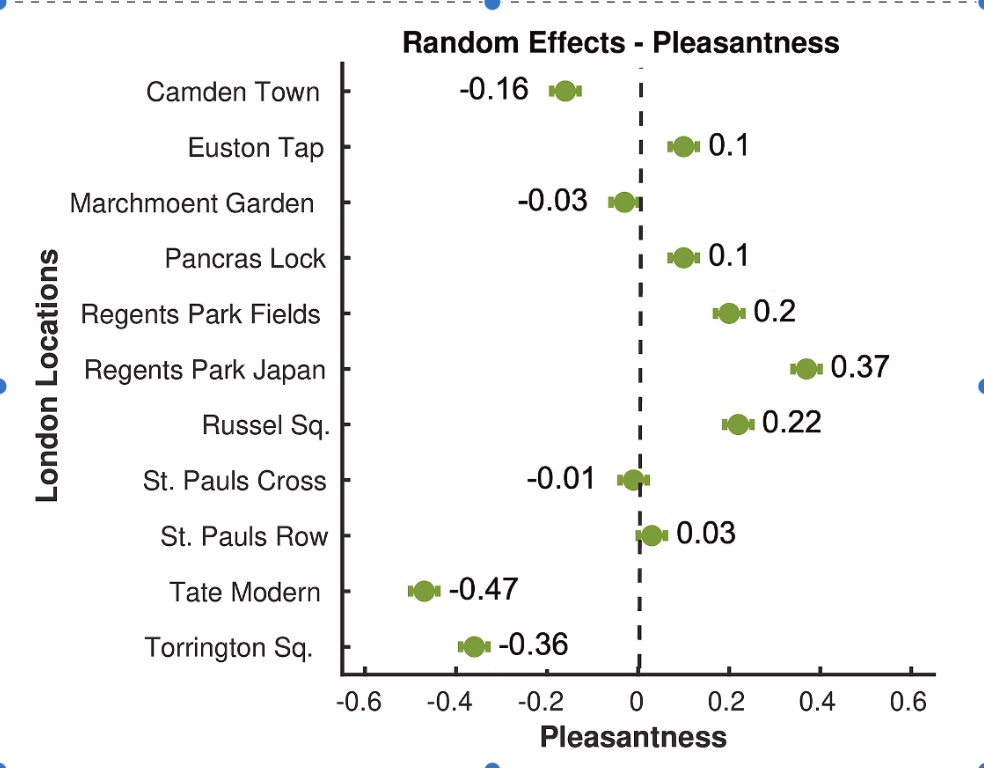
\includegraphics[width=\linewidth]{Figures/whoRandPl.jpg}
  \end{minipage}%
  \begin{minipage}{.5\textwidth}
    \centering
    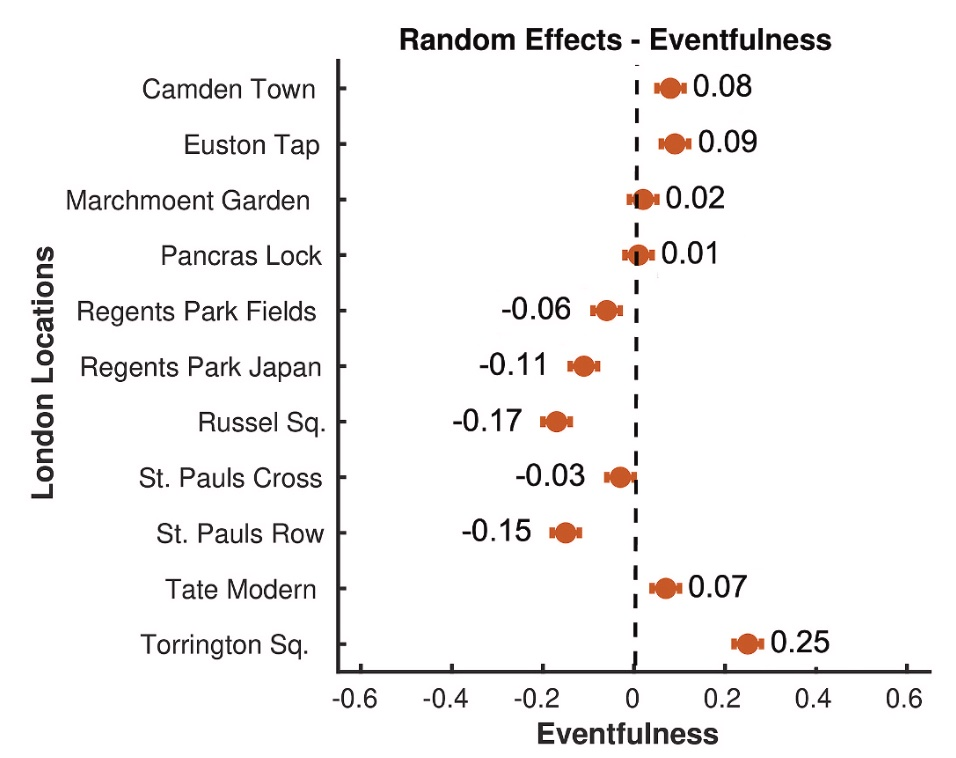
\includegraphics[width=\linewidth]{Figures/whoRandEv.jpg}
  \end{minipage}
  \caption{The summary result demonstrated in the random-effects figures gives the average from the distribution of \gls{isopl} across locations.\label{fig:whoRand}}

\end{figure}


\subsubsection*{Occupation status}
According to my findings, occupation status, in particular `retirement' and to a lesser degree, gender (male) were important factors in the pattern of soundscape assessments. It is worthwhile to highlight that `retirement' factor could potentially be a proxy for age (>65) and gender (male). In order to further investigate the effect which the inclusion of occupational status had on the model building process, I re-ran the stepwise feature selection, this time without including occupation status in the initial model. This allowed me to determine whether other features (namely age and gender) would be finally selected and how they would interact within the model. The results of this process are given in \cref{tab:whoLMER2}.

%  \afterpage{
\begin{landscape}
  \begin{table}[hp]
    \centering
    \caption{Linear mixed effects model resulting from the feature selection process when the initial model does not include occupational status. **$p<0.01$, *$p>0.05$  \label{tab:whoLMER2}}
    % \resizebox{\textwidth}{!}{%

    \begin{tabular}{@{}lcccccc@{}}
      \toprule
                         & \multicolumn{3}{c|}{\textbf{ISOPleasant}} & \multicolumn{3}{c}{\textbf{ISOEventful}}                                                                                                      \\
      \midrule
      \textbf{Predictor} & \textbf{Estimates}                        & \textbf{Std. Est.}                       & \multicolumn{1}{c|}{\textbf{95\% CI}} & \textbf{Estimates} & \textbf{Std. Est.} & \textbf{95\% CI} \\
      WHO-5              & 0.001**                                   & \textbf{0.03}                            & \multicolumn{1}{c|}{0.01, 0.05}       & -                  & -                  & -                \\
      Age                & \textbf{0.001*}                           & \textbf{0.02}                            & \multicolumn{1}{c|}{0.001, 0.04}      & \textbf{-0.001**}  & \textbf{-0.03}     & -0.05, -0.01     \\
      Gender (male)      & -                                         & -                                        & \multicolumn{1}{c|}{-}                & \textbf{-0.04*}    & \textbf{-0.04}     & -0.07, -0.001    \\
      Ethnicity          & -                                         & -                                        & \multicolumn{1}{c|}{-}                & \textbf{-0.09**}   & \textbf{-0.09}     & 0.03, 0.14       \\
      \midrule
      \multicolumn{7}{l}{\textbf{Random Effects}}                                                                                                                                                                    \\
      \midrule
      $\sigma^2$         & \multicolumn{3}{l|}{0.11}                 & \multicolumn{3}{l}{0.08}                                                                                                                      \\
      $\tau_{00}$        & \multicolumn{3}{l|}{0.06$_{Location}$}    & \multicolumn{3}{l}{0.01$_{Location}$}                                                                                                         \\
      ICC                & \multicolumn{3}{l|}{0.34}                 & \multicolumn{3}{l}{0.14}                                                                                                                      \\
      N                  & \multicolumn{3}{l|}{11}                   & \multicolumn{3}{l}{11}                                                                                                                        \\
      \midrule
      Observations       & \multicolumn{3}{l|}{1134}                 & \multicolumn{3}{l}{1134}                                                                                                                      \\
      Marginal $R^2$/%
      Conditional $R^2$  & \multicolumn{3}{l|}{0.009 / 0.345}        & \multicolumn{3}{l}{0.023 / 0.165}                                                                                                             \\
      AIC                & \multicolumn{3}{l|}{778.271}              & \multicolumn{3}{l}{456.130}                                                                                                                   \\
      \bottomrule
    \end{tabular}
    % }
  \end{table}
\end{landscape}
% }

Age (\gls{isopl}: $\beta=0.02, p=0.05$; \gls{isoev}: $\beta=-0.03, p=0.01$) and gender (\gls{isoev}: $\beta=-0.04, p=0.05$) then came out as significant, as shown in \cref{tab:whoLMER2}. This would indicate that occupation status, particularly `retirement', represents a group of older male individuals. Even though incorporation of occupation into the model complicates the interpretation of the outcome, it results in a slightly better fitting model ($R^2_c$ for \gls{isopl} (0.354) and \gls{isoev} (0.181)) relative to 0.345 for \gls{isopl} and 0.165 for \gls{isoev} in the model without occupation status, which is why it is selected by the feature selection process. These findings are in line with previous research, suggesting significant differences among age groups in the soundscape of different acoustic environments \citep{Ren2016Soundscape,Yang2005Acoustic}. My findings imply that an increase in age leads to an increase in the positive appraisal of the soundscape pleasantness. This is supported by a study by \citet{Aydin2016Assessment} in which they found that soundscape pleasantness reported by young individuals was significantly lower than the other age groups.

Age could potentially highlight the contextual role of the acoustic environment. Past experiences, memories, and even traumas give a particular context to our perception and shape the soundscape, making individual perception highly diverse, depending on the content of experience/memory. While the increase in age can lead to appreciating different sound elements, lower age seems to be related to more arousing and vibrant sounds \citep{Yang2005Acoustic}.

Like age, gender was found to be associated with the soundscape eventfulness. Past works have also reported that there are gender-related discrepancies in soundscape \citep{Croome1977Noise,Yang2005Acoustic}. These differences may be an indication of different auditory processing across genders.

In order to further investigate the effect which the inclusion of occupational status had on the model building process, I re-ran the stepwise feature selection, this time without including occupation status in the initial model. This allowed me to determine whether other features (namely age and gender) would be finally selected and how they would interact within the model. The results of this process are given in \cref{tab:whoLMER2}.



\subsubsection*{Soundscape pleasantness and eventfulness differences among locations}

The pleasantness and eventfulness were significantly different among locations. Pleasantness appeared to be highest in locations dominated by nature sounds (i.e. Regents Park Japan). In agreement with my results, \citet{Payne2013production} referred to the pleasantness dimension of the soundscape as the positive perception of natural places as well as the restorative capacity of the soundscape. \citet{Zhang2014Research} also reported a significant impact of natural soundscape on individuals' restorative experiences and boosting pleasantness. In the study by \citet{Axelsson2010principal} participants reported that the sound excerpts of natural components are more pleasant than human and technical sounds. Unlike pleasantness, the eventfulness increased the most in locations with dominant traffic and other sounds (i.e. Euston Tap). These findings are supported by previous research done by \citet{Bradley2000Emotion} and \citet{Hume2013Physiological}. In both studies, unnatural and urban sound-clips (i.e. fire engine siren and traffic noise), inherent in the traffic-dominant locations in this chapter, were rated highest in arousal and lowest in the pleasantness dimension. As formerly mentioned by \citet{Erfanian2019Psychophysiological}, throughout the soundscape literature, arousal has been applied as the equivalent of eventfulness and indicated on the Y-axis of the circumplex model \citep{Axelsson2010principal,Erfanian2019Psychophysiological}.


These results insinuate the notion that there are multiple primary factors \citep{Bradley2000Emotion} that contribute to the perception of the acoustic environment which should be considered important by urban designers and policymakers. It is expected that understanding these factors will provide multidimensional knowledge in guiding the implementation of the technological infrastructure of smart cities.

\section{Discussion}
\copied{For this chapter, data of 1134 participants across 11 locations in London were included in the analysis.} The goal of this chapter was to determine to what extent secondary factors mediate soundscape perception, and to highlight which of these secondary factors are important to consider. 

As expected, the majority of the total variance in the perceptual ratings is explained by the location-level differences (i.e. overall sound level) which represent primary contributing factors to the acoustic environment (see \citep{McDermott2012Auditory}) and other non-acoustic factors. Approximately 3\% of the variance is then explained by the combination of personal factors, which represent secondary contributing factors as defined by McDermott. Although the variance explained by these secondary factors is small compared to the primary factors, they are still found to contribute significantly. Furthermore an additional 3 percentage points of explained variance would represent a meaningful improvement in the performance of predictive soundscape models based on in-situ measurements of varying soundscape types \citep{Lionello2020systematic} and should therefore be considered when constructing these models.



\copied{My initial assumption was that an increased level of psychological well-being is associated with increased pleasantness and eventfulness assessments of the soundscape. Although the results showed that psychological well-being was positively associated with pleasantness, it was negatively associated with eventfulness in males and individuals that did not report their occupation.}

\copied{Then I hypothesized that differences in soundscape assessments are associated with demographic features. The results suport this hypothesis to a certain degree. Occupation and gender appeared to be strong demographic factors influencing the pleasantness and eventfulness assessment. Retirement as occupation status showed to be positively attribute to pleasantness and negatively to the eventfulness assessment. Further investigation revealed that the occupation (no occupation reported) was negatively associated with pleasantness and gender (male) was negatively associated with eventfulness, whereas unemployment was positively associated with eventfulness.}



\subsection{Incorporating personal factors}
Although, as \citet{Droumeva2021sound} points out, each individual brings their own cultural and subjective aspects of listening to the stage of urban sound, when attempting to characterise the soundscape of a space, it is not a particular individual's aspects we should be concerned with. That individual forms a part of the collective perception of the space. Their cultural and subjective (i.e. personal) aspects mitigate their perception, but this perception then forms only a single component of the collective perception. How then should we consider these personal factors? Surely there is no suggestion to disregard their influence and importance within the soundscape approach? In my view, there are two approaches:

\begin{enumerate}
  \item Incorporate these personal factors as demographic statistics of a location; or
  \item An agent-based approach where each individual likely to use the space is simulated and modelled with their personal factors to then be included in the collective perception.
\end{enumerate}

Let's look at how these two approaches would be implemented into the multilevel acoustics-based predictive model, such as those presented in \crefrange{ch:mlmann}{ch:lockdown}.

%TODO: Expand
\subsubsection{Approach 1}
In the first, the demographic breakdown of the space under investigation is estimated, either through a census or by the designers' desired use case. This demographic breakdown can then be compared to the results presented above \citep{Erfanian2021Psychological} to derive weighting factors which adjust the predicted soundscape assessment. For instance, the results suggest that retired persons perceive the soundscape as \draft{XX\% or amount [need to check with results]} less pleasant than others. If the particular space under investigation has a large proportion of retired persons, say 65\% we could then apply an adjustment to the initial personal-factors-agnostic prediction to reflect this tendency. In this example, an initial location-level \gls{isopl} prediction of 0.36, with a 65\% retired population would be corrected by \draft{-XX [0.65 x result]} for a final demographics-corrected \gls{isopl} prediction of \draft{XX}.

\subsubsection{Approach 2}

\subsubsection{Benefits and downsides of each approach}

\section{Conclusion}
\draft{Rewrite to put in context of the predictive model framework}
In this chapter, I conducted a linear mixed-effects model to show the associations of psychological well-being and demographic factors with the soundscape pleasantness and eventfulness. The findings indicate that psychological well-being is positively associated with pleasantness and negatively associated with eventfulness in males and individuals that did not report their occupations. I further demonstrated that the occupational status, in particular retirement as a proxy of age and gender, was related to the perceptions of pleasantness and eventfulness. In total, these personal factors were shown to account for 1.4\% of the variance for pleasantness and 3.9\% of the variance for eventfulness. The findings of this chapter offer empirical grounds for developing and advancing theories on the influence of psychological well-being and demographic characteristics on the perception of the acoustic environment.

